% ================================================================== A
\chapter{Proposal Action Register}\label{app:register}
\begingroup\small
\begin{longtable}{L{0.45cm} L{1.4cm} L{3.0cm} L{4.15cm} L{1.35cm} L{2.3cm}}
\caption{Complete proposal action register}\label{tab:registerfull}\\
\toprule
\textbf{No.} & \textbf{Source} & \textbf{Feedback / required change} & \textbf{Action taken} & \textbf{Status} & \textbf{Evidence}\\
\midrule\endfirsthead
\toprule
\textbf{No.} & \textbf{Source} & \textbf{Feedback / required change} & \textbf{Action taken} & \textbf{Status} & \textbf{Evidence}\\
\midrule\endhead
\bottomrule\endlastfoot
P1 & Proposal panel & Bring clarity to intended goals. & Goals restated: light, fast, integrated platform plus fair, cheap crop-type models; crop mapping, GIS integration and ``real-time'' defined; objectives have measurable targets. & Done & Section~\ref{sec:goals}\\
P2 & Proposal panel & Improve evaluation metrics. & Evaluation criteria rewritten per concern with metric, target and measured value; spatial block protocol with intervals for models. & Done & Table~\ref{tab:evalcriteria}, Sec.~\ref{sec:protocol}\\
P3 & Proposal panel & Measure the real challenges: computational performance, lightweight system, usability; usability, performance and integration are the main concerns. & Performance benchmark; CPU cost, size and RAM for 11 models; integration tests; usability checked against NFR-U1--U3; user study planned. & Partly done & Tables~\ref{tab:benchmark}, \ref{tab:cost}, \ref{tab:evalcriteria}\\
P4 & Proposal panel & Analyse complexity and resource requirements of the complete workflow beforehand. & Each stage measured for time, peak RAM and storage; baseline crop-type model (1.57~GB, 3.1~GB RAM) identified as the bottleneck; LightGBM (1.98~MB, 549~MB RAM) selected. & Done & Table~\ref{tab:resources}\\
P5 & Proposal panel & Running the entire process in a single flow may not be practical. & Separate queued stages in background workers, one model at a time in dependency order; per-step progress and errors; workers scale out. & Done & Sec.~\ref{sec:feasibility}, Fig.~\ref{fig:seq}\\
P6 & Proposal panel & Huge datasets are not easy to load and use together. & Results kept as COGs; only visible tiles sent (337~KB per screen against 43.3~MB); boundaries as PMTiles; one layer catalogue. & Done & Table~\ref{tab:benchmark}, Fig.~\ref{fig:benchmark}\\
P7 & Proposal panel & Work on presentation skills. & Fixed demonstration script on the running system; each member presents their own track; rehearsals before each evaluation. & In progress & Sec.~\ref{sec:demo}\\
T1 & Team review & Uploads were recorded but never analysed. & Processing pipeline with validation, COG conversion and background model runs; 57~s upload to map. & Done & TC-11, Fig.~\ref{fig:seq}\\
T2 & Team review & Dashboard used hand-written sample data. & Statistics computed from real result rasters and stored in PostGIS. & Done & TC-07, Fig.~\ref{fig:shot-dashboard}\\
T3 & Team review & First evaluation used a random pixel split. & Spatial block split with buffer, validation-only choices, block bootstrap intervals. & Done & Sec.~\ref{sec:protocol}\\
T4 & Team review & Models will change over the project. & Plug-in registry with manifests and dependency graph; add-a-model test. & Done & TC-03\\
T5 & Team review & Slide iteration plan outdated. & Two-track iteration plan with four iterations. & Done & Table~\ref{tab:iterations}\\
T6 & Team review & Use the original prototype's look in the new portal. & Portal restyled after the prototype (home page, workspace, panels). & Done & Figs.~\ref{fig:shot-home}, \ref{fig:shot-map}\\
T7 & Team review & Integrate the selected crop-type pipeline into the platform. & Planned as first item of Iteration 2. & Open & Section~\ref{sec:it2plan}\\
T8 & Team review & Like-for-like comparison with Tran et al. & CDL confidence rule and class alignment in Iteration 2. & Open & Section~\ref{sec:papers}\\
T9 & Team review & Usability study with users. & Task-based study with SUS questionnaire. & Open & Section~\ref{sec:it2plan}\\
\end{longtable}
\endgroup

% ================================================================== B
\chapter{Detailed Requirements}\label{app:requirements}
\begin{table}[htbp]
\centering\small
\caption{Remaining use cases in brief}
\label{tab:ucbrief}
\begin{tabularx}{\textwidth}{L{1.1cm} L{2.6cm} Y L{2.6cm}}
\toprule
\textbf{ID} & \textbf{Actor} & \textbf{Main flow} & \textbf{Alternative flows}\\
\midrule
UC-03 & Agricultural Analyst & Choose a crop in the Filter chip or click a crop in the ranking; map shows only that crop; type a crop name to search field regions and click one to fly to it. & No match: ``No field regions match''.\\
UC-04 & Agricultural Analyst & Open Dashboard; choose area, layer and unit; read classified area, class shares, breakdown table and model accuracy. & Area without categorical layers: empty state.\\
UC-06 & GIS Analyst & After an upload or run, the Processing page polls the job and shows steps, progress and messages; on completion links to the Live Map. & Failed job: reason shown; link to analyse another image.\\
UC-07 & GIS Analyst & Choose an image already in GeoCrop and models; a run job starts; layers are added. & Unknown model or missing dependency: readable error.\\
UC-08 & Any user & Open Models; read status, inputs, outputs, valid regions, accuracy and F1 per class. & Registry errors listed.\\
UC-09 & Any user & Create an account (all fields, matching passwords, unique username and email) or log in. & Duplicate username or email; wrong password.\\
UC-10 & Platform Developer & Open System Status; see health of database, queue, storage, tiles and registry, plus configuration notes. & Failed service shown in red with detail.\\
UC-12 & Processing Worker & Take a job from the queue; run ingest or model steps; publish layers and statistics; update progress. & Retry on transient errors; mark failed with reason.\\
\bottomrule
\end{tabularx}
\end{table}

\begin{table}[htbp]
\centering\small
\caption{Requirement priority and status}
\label{tab:reqstatus}
\begin{tabularx}{\textwidth}{L{2.6cm} L{1.6cm} Y}
\toprule
\textbf{Requirement} & \textbf{Priority} & \textbf{Status at mid-term}\\
\midrule
FR-ING-01..07 & Must & Implemented and tested (FR-ING-06 stores location as area name and capture date on the image)\\
FR-REG-01..05 & Must & Implemented and tested\\
FR-MAP-01..02 & Must & Baseline implemented; selected pipeline in Iteration 2\\
FR-CAT-01..04 & Must & Implemented; FR-CAT-03 uses derived field regions\\
FR-VIS-01..08 & Must & Implemented and tested\\
FR-AUT-01 & Should & Implemented; optional by configuration\\
NFR-P1, P2, P4 & Must & Met (Table~\ref{tab:acceptance})\\
NFR-P3 & Should & Not yet measured\\
NFR-P5 & Must & Met by the selected model (2~MB, CPU); integration pending\\
NFR-R1..R4, U1..U4, S1..S5 & Must & Implemented; S3 tile-level authorisation partial\\
\bottomrule
\end{tabularx}
\end{table}

% ================================================================== C
\chapter{Detailed Test Cases}\label{app:tests}
\begingroup\small
\begin{longtable}{L{1.0cm} L{3.0cm} L{4.3cm} L{3.3cm} L{1.1cm}}
\caption{Detailed test cases}\label{tab:testdetail}\\
\toprule
\textbf{ID} & \textbf{Preconditions / input} & \textbf{Steps} & \textbf{Expected result} & \textbf{Result}\\
\midrule\endfirsthead
\toprule
\textbf{ID} & \textbf{Preconditions / input} & \textbf{Steps} & \textbf{Expected result} & \textbf{Result}\\
\midrule\endhead
\bottomrule\endlastfoot
TC-01 & Built-in model folders & Load the registry & No errors; cropland, croptype, boundary, yield, NDVI found & Pass\\
TC-02 & Registry & Plan \code{croptype}; plan \code{yield} & [cropland, croptype]; [cropland, croptype, yield]; unknown and cyclic plans give readable errors & Pass\\
TC-03 & Copy of the NDVI template with a new key & Load both folders; plan and run on a 64$\times$64 synthetic 7-band raster & Model discovered; one float32 output, values $\leq$ 1 & Pass\\
TC-04 & Yield placeholder & Run on synthetic raster & Status ``not available''; no files & Pass\\
TC-05 & Seeded AOI1 layers & Request a z12 tile of each raster layer & 200, PNG 256$\times$256, immutable cache header & Pass\\
TC-06 & Same & Request a tile outside the data; repeat a tile & 204; second request \code{X-Cache-Status: HIT} & Pass\\
TC-07 & Crop-type layer & \code{GET /stats?layer=} & 14 classes; areas sum to total; shares & Pass\\
TC-08 & Crop-type and cropland visible & \code{GET /point} at a pivot field; click in browser & Labels returned (Alfalfa / Cropland; Spring Wheat) & Pass\\
TC-09 & Live Map & Choose ``Apples'' in Filter & Only apple pixels remain & Pass\\
TC-10 & Field regions layer & Range request with Origin header to the PMTiles URL & 206 Partial Content; CORS header & Pass\\
TC-11 & AOI1 Sentinel-2 GeoTIFF (7 bands) & Signed PUT; complete with cropland and crop type; poll job & Done in under 2 min; 6 steps done; layers listed & Pass (57~s)\\
TC-12 & Existing image & Re-run NDVI from Analyze Imagery & Processing page shows done; layer listed & Pass\\
TC-13 & 1-band CDL GeoTIFF & Upload and complete & Job failed with band-count reason & Pass\\
TC-14 & Running stack & \code{make benchmark} & Under 1~MB per screen; cold under 300~ms; cached under 50~ms & Pass\\
TC-15 & Stopped stack & \code{docker compose up -d}; \code{GET /health} & All services healthy; status ok & Pass\\
\end{longtable}
\endgroup

\begingroup\small
\begin{longtable}{L{3.2cm} r r r r r r}
\caption{AOI1 per-class results (improved pipeline with neighbour vote; test pixels)}\label{tab:perclass}\\
\toprule
\textbf{Class} & \textbf{Test px} & \textbf{On edges} & \textbf{F1 bench.} & \textbf{F1 final} & \textbf{Recall int.} & \textbf{Recall edge}\\
\midrule\endfirsthead
\toprule
\textbf{Class} & \textbf{Test px} & \textbf{On edges} & \textbf{F1 bench.} & \textbf{F1 final} & \textbf{Recall int.} & \textbf{Recall edge}\\
\midrule\endhead
\bottomrule\endlastfoot
Alfalfa & 19,789 & 40.0\% & 0.829 & 0.845 & 0.960 & 0.504\\
Corn & 14,830 & 41.5\% & 0.821 & 0.819 & 0.965 & 0.637\\
Potatoes & 14,277 & 35.1\% & 0.883 & 0.860 & 0.971 & 0.684\\
Other Hay & 9,061 & 58.6\% & 0.707 & 0.722 & 0.949 & 0.535\\
Winter Wheat & 7,703 & 47.3\% & 0.774 & 0.792 & 0.967 & 0.598\\
Apples & 7,698 & 60.6\% & 0.620 & 0.644 & 0.866 & 0.415\\
Sweet Corn & 7,149 & 44.1\% & 0.682 & 0.709 & 0.963 & 0.584\\
Dry Beans & 5,345 & 50.8\% & 0.745 & 0.743 & 0.938 & 0.714\\
Other (rare) & 3,598 & 82.6\% & 0.239 & 0.287 & 0.595 & 0.110\\
Peas & 2,751 & 72.0\% & 0.509 & 0.538 & 0.858 & 0.589\\
Sod/Grass Seed & 2,490 & 42.2\% & 0.715 & 0.706 & 0.951 & 0.731\\
Onions & 2,292 & 25.9\% & 0.911 & 0.913 & 0.998 & 0.737\\
Spring Wheat & 1,506 & 51.3\% & 0.550 & 0.741 & 0.997 & 0.429\\
Fallow/Idle & 749 & 99.5\% & 0.269 & 0.289 & n/a & 0.517\\
\end{longtable}
\endgroup

\begin{table}[htbp]
\centering\small
\caption{AOI2 per-class results (improved pipeline with neighbour vote)}
\label{tab:perclass2}
\begin{tabular}{L{3.2cm} r r r r r}
\toprule
\textbf{Class} & \textbf{Test px} & \textbf{Recall} & \textbf{Precision} & \textbf{F1 final} & \textbf{F1 bench.}\\
\midrule
Canola & 52,527 & 0.979 & 0.975 & 0.977 & 0.972\\
Spring Wheat & 47,912 & 0.921 & 0.955 & 0.938 & 0.925\\
Soybeans & 20,268 & 0.912 & 0.902 & 0.907 & 0.901\\
Fallow/Idle & 14,051 & 0.840 & 0.841 & 0.840 & 0.817\\
Barley & 3,255 & 0.614 & 0.740 & 0.671 & 0.581\\
Dry Beans & 2,584 & 0.886 & 0.825 & 0.854 & 0.792\\
Peas & 2,255 & 0.875 & 0.620 & 0.726 & 0.707\\
Other (rare) & 1,259 & 0.659 & 0.414 & 0.509 & 0.428\\
Sunflower & 811 & 0.783 & 0.837 & 0.809 & 0.712\\
\bottomrule
\end{tabular}
\end{table}

\begin{table}[htbp]
\centering\small
\caption{Fair reporting of AOI1 accuracy by subset of test pixels (accuracy \% / macro-F1)}
\label{tab:subsets}
\begin{tabular}{L{5.6cm} r c c c}
\toprule
\textbf{Pixels counted} & \textbf{Share} & \textbf{Benchmark} & \textbf{Improved} & \textbf{+ vote}\\
\midrule
All test pixels (headline) & 100.0\% & 74.1 / 0.661 & 75.6 / 0.685 & 76.1 / 0.686\\
Same-label patch $\geq$ 10 px (0.9 ha) & 84.5\% & 83.3 / 0.725 & 85.0 / 0.756 & 86.4 / 0.771\\
Same-label patch $\geq$ 50 px (4.5 ha) & 79.2\% & 86.6 / 0.807 & 88.3 / 0.849 & 90.0 / 0.867\\
Interior pixels (3$\times$3 same label) & 53.0\% & 93.8 / 0.825 & 94.9 / 0.853 & 95.2 / 0.856\\
Deep interior (5$\times$5 same label) & 36.2\% & 96.4 / 0.927 & 97.1 / 0.952 & 97.4 / 0.955\\
\bottomrule
\end{tabular}
\end{table}
Subsets use only the reference labels, never model output; they describe where errors are and are not
a better score. The all-pixel number is always quoted first.

% ================================================================== D
\chapter{Repository and Contribution Evidence}\label{app:repo}
\begin{table}[htbp]
\centering\small
\caption[Platform repository history (geocrop-platform, branch main)]{Platform repository history (\code{geocrop-platform}, branch \code{main})}
\label{tab:commits}
\begin{tabularx}{\textwidth}{L{1.8cm} L{1.9cm} Y}
\toprule
\textbf{Commit} & \textbf{Date} & \textbf{Message}\\
\midrule
\code{f056a54} & 2026-10-14 & Step 0: repo skeleton, env example, data fetch script\\
\code{1ec3dc9} & 2026-10-14 & Backend, model registry, tile service, React app, compose stack and docs\\
\code{fae4751} & 2026-10-14 & Initial migration, Docker fixes, MapLibre worker, verified end to end with benchmark\\
\code{efc3c68} & 2026-10-14 & Retry MinIO connection in bucket init (fixes cold-start race)\\
\code{1e416ed} & 2026-10-14 & Open straight to the map without sign-in; fix NaN nodata and stale page cache\\
\code{4c631c9} & 2026-10-14 & Restyle the web app after the original GeoCrop prototype\\
\bottomrule
\end{tabularx}
\end{table}

\begin{table}[htbp]
\centering\small
\caption{Prototype repository history (proposal stage)}
\label{tab:protocommits}
\begin{tabularx}{\textwidth}{L{1.8cm} L{1.9cm} Y}
\toprule
\textbf{Commit} & \textbf{Date} & \textbf{Message}\\
\midrule
\code{f10912e} & 2026-09-01 & Initial Django project\\
\code{4dfe6b3} & 2026-09-05 & Update frontend to look slight professional\\
\code{02f9e00} & 2026-09-05 & Add render setup\\
\code{bab4d9e} & 2026-09-05 & Add Django dependencies\\
\code{0788e6f} & 2026-09-05 & Trigger Vercel deployment\\
\code{b4ed861} & 2026-09-05 & Add requirements.txt for Render deployment\\
\code{b9b63cd} & 2026-09-08 & Add changes\\
\code{3760eae} & 2026-09-08 & Add changes to the crop result file\\
\bottomrule
\end{tabularx}
\end{table}

\textbf{Platform repository structure.}
\begin{verbatim}
geocrop-platform/
  backend/   app/ (api, core, db, services, workers, cli)
             model_registry/, alembic/, tests/
  tiles/     TiTiler-based tile service
  web/       React app and nginx.conf
  ml/        extended training scripts
  tools/     to_cog.py, build_boundaries.py,
             benchmark_tiles.py
  infra/     MinIO initialisation, Nginx reference
  docs/      architecture, status, upgrade path, report
  docker-compose.yml, Makefile, .env.example
\end{verbatim}

% ================================================================== E
\chapter{Additional Design Diagrams}\label{app:diagrams}
\begin{figure}[htbp]
\centering
\begin{tikzpicture}[every node/.style={font=\scriptsize}]
\node[box, text width=4.6cm] (web) at (0,0) {\textbf{web} (Nginx 1.27)\\built React app, proxy, tile cache; port 8080};
\node[box, text width=3.6cm] (api) at (-4.2,-2.0) {\textbf{api} (FastAPI)\\Alembic upgrade at start; port 8000};
\node[box, text width=3.2cm] (tiles) at (4.2,-2.0) {\textbf{tiles} (TiTiler)\\2 workers; port 8001};
\node[box, text width=3.4cm] (worker) at (0,-4.0) {\textbf{worker} (Celery)\\queues: ingest, models};
\node[box, text width=2.9cm] (init) at (4.2,-4.0) {\textbf{minio-init}\\creates bucket; public read for vectors};
\node[dbox, minimum width=3.0cm] (pg) at (-4.2,-6.2) {\textbf{postgres}\\PostGIS 16-3.4; 5432};
\node[dbox, minimum width=2.4cm] (redis) at (0,-6.2) {\textbf{redis} 7\\broker};
\node[dbox, minimum width=2.8cm] (minio) at (4.2,-6.2) {\textbf{minio} (S3)\\9000 / 9001};
\node[box, text width=11.6cm, fill=gray!8] (vol) at (0,-7.75) {Named volumes: pgdata (postgres), miniodata (minio), nginxcache (web); bind mount ./data for sample imagery};
\draw[arr] (web) -- (api); \draw[arr] (web) -- (tiles);
\draw[arr] (api) -- node[lbl]{SQL} (pg);
\draw[darr] (api.south) ++(1.0,0) |- node[lbl,pos=0.75]{enqueue} (worker.west);
\draw[arr] (worker) -- (redis);
\draw[arr] (worker.south west) -- (pg.north east);
\draw[arr] (worker.south east) -- (minio.north west);
\draw[arr] (tiles.east) -- ++(1.0,0) |- node[lbl,pos=0.25]{range reads} (minio.east);
\draw[darr] (init) -- node[lbl]{setup} (minio);
\end{tikzpicture}
\caption{Deployment view of the Docker Compose stack}
\label{fig:deploy}
\end{figure}

\begin{figure}[htbp]
\centering
\begin{tikzpicture}[node distance=0.35cm, every node/.style={font=\scriptsize}]
\node[box, text width=2.3cm] (p1) {Plan models\\(topological sort)};
\node[box, text width=2.3cm, right=of p1] (p2) {Create run;\\build context};
\node[box, text width=2.3cm, right=of p2] (p3) {Validate input\\(bands, artifacts)};
\node[box, text width=2.3cm, right=of p3] (p4) {Run task\\(512 px windows)};
\node[box, text width=2.3cm, below=0.7cm of p4] (p5) {COG, upload,\\layer + statistics};
\node[box, text width=2.3cm, left=of p5] (p6) {Store metrics;\\step done};
\node[box, text width=2.3cm, left=of p6] (p7) {Next model or\\job done};
\node[box, text width=2.3cm, left=of p7, fill=red!6] (p8) {Fail job with\\reason};
\draw[arr] (p1)--(p2); \draw[arr] (p2)--(p3); \draw[arr] (p3)--(p4); \draw[arr] (p4)--(p5);
\draw[arr] (p5)--(p6); \draw[arr] (p6)--(p7);
\draw[darr] (p3.south) .. controls +(0,-0.9) and +(0.8,0.4) .. node[lbl,pos=0.5]{problems} (p8.north east);
\draw[darr] (p7.north) -- node[lbl,left]{more} (p7.north |- p2.south) -- (p2.south);
\end{tikzpicture}
\caption{Activity of a model run inside the worker}
\label{fig:activity}
\end{figure}

\begin{figure}[htbp]
\centering
\fbox{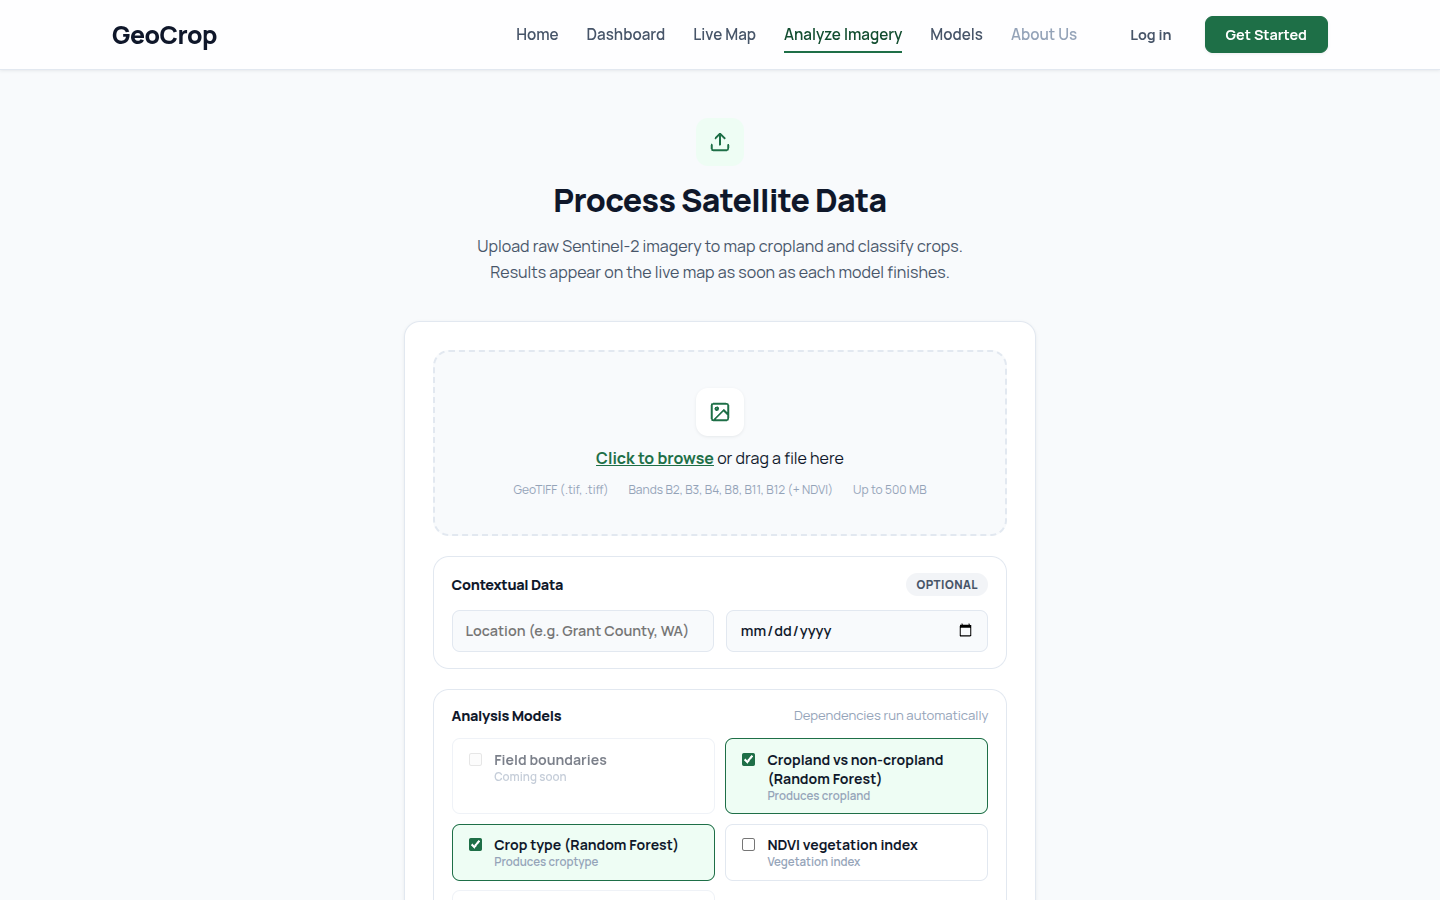
\includegraphics[width=0.88\textwidth]{figures/shot_analyze.png}}
\caption{Analyze Imagery: drag-and-drop upload, contextual data and model selection}
\label{fig:shot-analyze}
\end{figure}

\begin{figure}[htbp]
\centering
\fbox{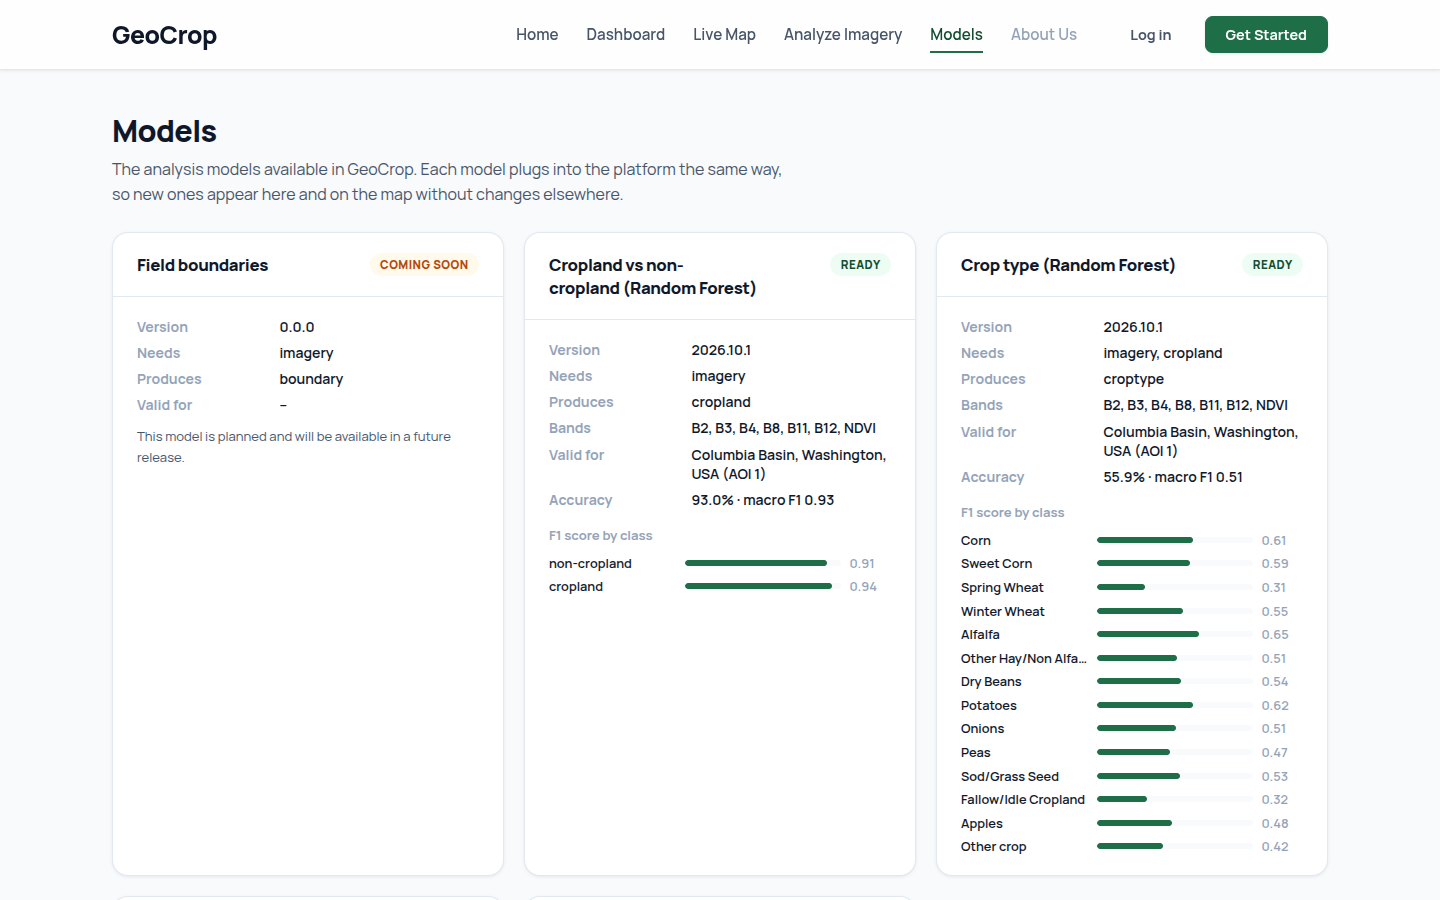
\includegraphics[width=0.88\textwidth]{figures/shot_models.png}}
\caption{Models page: registered models, status, accuracy and F1 per class}
\label{fig:shot-models}
\end{figure}

% ================================================================== F
\chapter{Meeting and Progress Evidence}\label{app:meetings}
\begin{table}[htbp]
\centering\small
\caption{Progress evidence from dated project artefacts}
\label{tab:progressevidence}
\begin{tabularx}{\textwidth}{L{2.4cm} Y L{4.2cm}}
\toprule
\textbf{Date (2026)} & \textbf{Progress} & \textbf{Artefact}\\
\midrule
1--8 Sep & Proposal-stage prototype implemented & Prototype repository commits\\
7--8 Sep & Proposal written & Proposal document and \LaTeX{} source\\
11 Sep & Proposal defence & Proposal slides (F26-155-GeoCrop)\\
14 Sep & Defence result: Approved with Minor Modifications; panel comments P1--P7 & FYP Committee e-mail\\
Sep--Oct & Crop-type experiments, runs 1--3 & Research notebooks\\
14 Oct & Crop-type results and paper comparison & Results report (prepared by Saneed Ullah)\\
14 Oct & Platform architecture implemented and verified & Platform repository commits; benchmark\\
15 Oct & Workflow resource measurement (P4) & Measurement script; Table~\ref{tab:resources}\\
15 Oct & Mid-report & This document\\
\bottomrule
\end{tabularx}
\end{table}

\begin{table}[htbp]
\centering\small
\caption{Supervisor meeting record (to be completed and signed by the team)}
\label{tab:meetings}
\begin{tabularx}{\textwidth}{L{2.0cm} L{3.0cm} Y L{2.6cm}}
\toprule
\textbf{Date} & \textbf{Attendees} & \textbf{Discussion and decisions} & \textbf{Supervisor signature}\\
\midrule
 & & & \\[0.8cm]
 & & & \\[0.8cm]
 & & & \\[0.8cm]
\bottomrule
\end{tabularx}
\end{table}

Open questions prepared for the supervisors: (1) whether LightGBM with neighbourhood inputs and a
3$\times$3 vote is accepted as GeoCrop's crop-type model; (2) whether the final comparison with the
papers should use the CDL confidence filter, reported next to the all-pixel score; (3) whether
field-level classification with field boundaries or the cross-area test should come first.
